\documentclass[aspectratio=169]{beamer}
\usepackage[utf8]{inputenc} % codificacao de caracteres
\usepackage[T1]{fontenc}    % codificacao de fontes
\usepackage[english]{babel}  % idioma
\usepackage{graphics,amssymb,amsfonts,amsmath,xfrac}
\usepackage{tikz}
\usepackage{enumerate,hyperref}
\usepackage{palatino}	% Fonte sem serifa
\usepackage{ragged2e}	% Paragrafo justificado
%\usepackage{minted}	% Highlight para codigos de programacao
\usepackage{booktabs} % tabelas
\usepackage{multicol}
\usepackage{multirow}
%\usepackage[table]{xcolor}


% Veja mais temas e cores em http://www.hartwork.org/beamer-theme-matrix/
\usetheme{Montpellier}         % tema
\usecolortheme{orchid}      % cores
\usefonttheme[onlymath]{serif} % fonte modo matematico
% Colocando numero de paginas no slide
\setbeamertemplate{footline}[frame number]



\DeclareGraphicsExtensions{.pdf,.jpg,.png} % compilamos apenas com pdflatex
\graphicspath{{figuras/}} % caminho onde as figuras estarao disponiveis




% ---------------------------------------------------------------------------- %
% T�tulo                                                                       %
% ---------------------------------------------------------------------------- %

\title[\sc{Teoria de Circuitos Eletrônicos 1}]{\LARGE Aula 15 - Exercise Class 5}
\author[Prof. Marcelino Andrade]{Prof. Marcelino Andrade}
\institute{Faculdade UnB Gama} % opcional
\date{\today}

\begin{document}
\justifying % Paragrafo justificado
\pagebreak
\small
\begin{frame}
  \titlepage
\end{frame}


% ----------------- NOVO SLIDE --------------------------------
\begin{frame}{Contents\newline}

\tableofcontents
\begin{center}	
     		Introduction to Electric Circuits by James A. Svoboda, Richard C. Dorf, 9th Edition			
\end{center}	
\end{frame}

% ----------------- NOVA SECÇÂO -----------------------------
\section{CHAPTER 7 Sinusoidal Steady-State Analysis}
% ----------------- NOVO SLIDE --------------------------------
\begin{frame}[fragile]
	\frametitle{Nodal Analysis}
\begin{tabular}{ll}
	\begin{columns}
		\begin{column}{1\textwidth}  %%<--- here
		\textbf{Example 10.1} - Find $i_x$ in the circuit below using  nodal analysis.\\
		\begin{center}
    			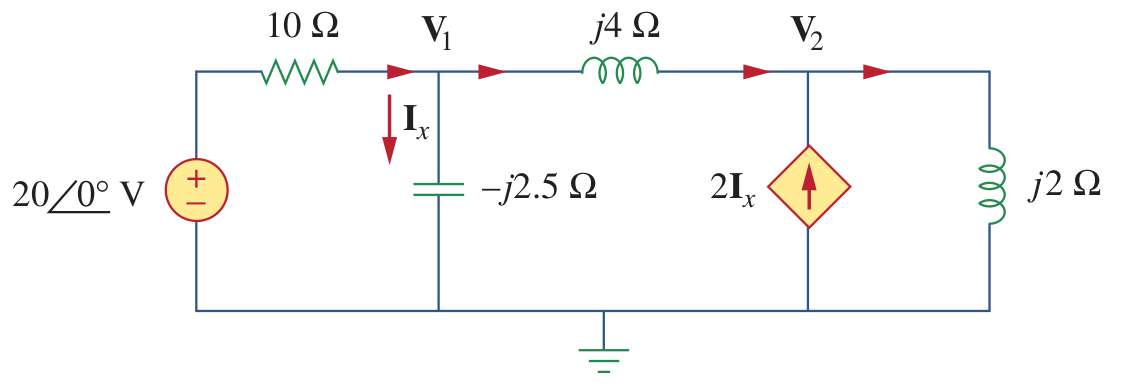
\includegraphics[height=3.6cm]{figure1.png}	
		\end{center}	
		\scalebox{0.8}{Answer: $7.59 \cos(4t+108.4^o)$.}
		\end{column}
	\end{columns}
\end{tabular}
\end{frame}

% ----------------- NOVO SLIDE --------------------------------
\begin{frame}[fragile]
	\frametitle{Mesh Analysis}
\begin{tabular}{ll}
	\begin{columns}
		\begin{column}{1\textwidth}  %%<--- here
		\textbf{Practice Problem 10.3} - Find $I_o$ in Fig. below using mesh analysis.\\
		\begin{center}
    			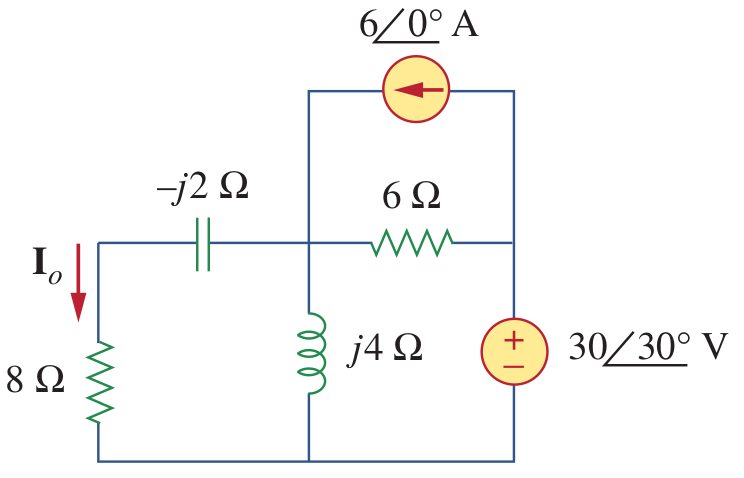
\includegraphics[height=3.6cm]{figure2.png}	
		\end{center}	
		\scalebox{0.8}{Answer: $I_0=3.582 \angle{65.45^o}$.}
		\end{column}
	\end{columns}
\end{tabular}
\end{frame}
% ----------------- NOVO SLIDE --------------------------------
\begin{frame}[fragile]
	\frametitle{Thevenin Equivalent Circuits}
\begin{tabular}{ll}
	\begin{columns}
		\begin{column}{1\textwidth}  %%<--- here
		\textbf{Practice Problem 10.9} - Determine the Thevenin equivalent of the circuit in Fig. below as seen
from the terminals a-b.\\
		\begin{center}
    			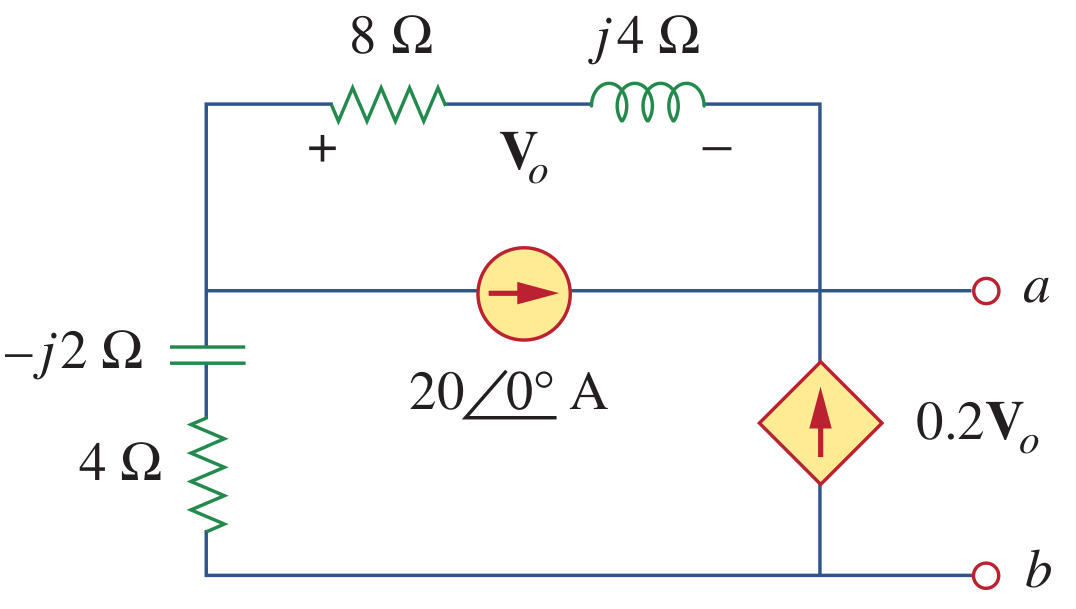
\includegraphics[height=3.6cm]{figure3.png}	
		\end{center}	
		\scalebox{0.8}{Answer: $\textbf{Z}_{Th}=4.473 \angle{-7.64^o}, \ \textbf{V}_{Th}=29.4 \angle{72.9^o}$ .}
		\end{column}
	\end{columns}
\end{tabular}
\end{frame}

% ----------------- NOVA SECÇÂO -----------------------------
\section{Diode}
% ----------------- NOVO SLIDE --------------------------------
\begin{frame}[fragile]
	\frametitle{Log Amplifier}
\begin{tabular}{ll}
	\begin{columns}
		\begin{column}{1\textwidth}  %%<--- here
		\textbf{Example} - Find the response $v_{out}$ in the circuit of
Fig. below.\\
		\begin{center}
    			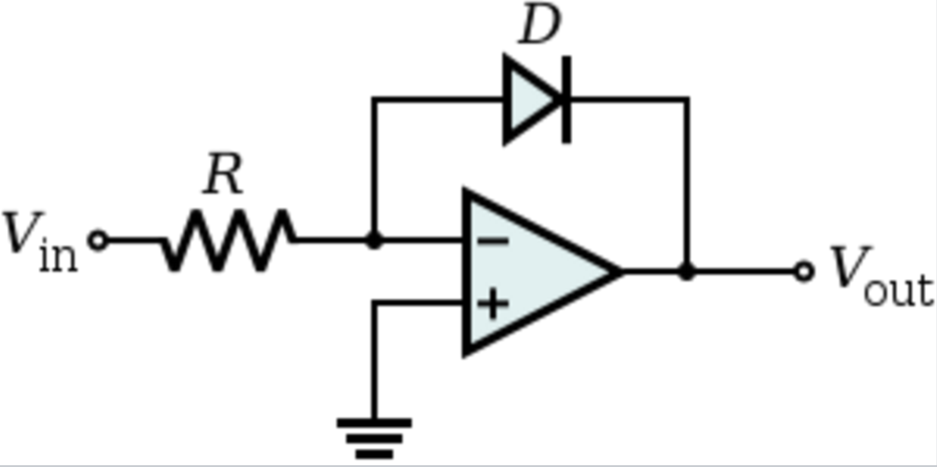
\includegraphics[height=3.6cm]{figure4.png}	
		\end{center}	
		\scalebox{0.8}{Answer: $v_{out}=-nv_t ln(\dfrac{v_{in}}{I_SR})($}
		\end{column}
	\end{columns}
\end{tabular}
\end{frame}




\end{document} 






